\def\DevnagVersion{2.15}\documentclass[12pt]{article}
\usepackage{devanagari}
\usepackage{cite}
\usepackage{pstricks}
\usepackage{pst-node}
\usepackage{pst-coil}
\usepackage{pst-rel-points}
\usepackage{graphics}
\usepackage{epsfig}
\usepackage{verbatim, hyperref, color}
\usepackage{float}
\usepackage[margin=3cm]{geometry}
\usepackage[T1]{fontenc}
\usepackage[english]{babel}
\setlength{\parindent}{0pt}
\setlength{\parskip}{0.2cm}
\topskip 0.0in

\title{Handling Anaphoras in multiple languages in the framework of Geometry Constructions}
\author{Jeetesh Mangwani \& Pankaj Prateek\\
	Advisor: Dr. Amitabh Mukherjee\\
        Dept. of Computer Science and Engineering\\
	Indian Institute of Technology, Kanpur, India\\
	\{jeeteshm, pratikkr, amit\} @ cse.iitk.ac.in}
\date{April 17, 2014}

\begin{document}
\maketitle
\begin{center}{\b \em ABSTRACT}\end{center}
{\em In this project, we take up the problem of handling anaphoras in multiple languages in the context of a language-independent interpreter for drawing geometric diagrams. We focus on ruler and compass based construction problems. We start with use cases and motivations on why such a system would be useful and wh ere deploying it would be fruitful. We give a brief tabulated review summary of related research work done on geometry related problems and point out the common trait that they lack the ability to decipher any problem/constraint expressed in a natural language. We, then, move to describe the design of the interpreter and the usage of cross-lingual alignment technique to provide the ability of language-independent interpretation. We briefly mention how the alignment model is utilised to realize the powerful translation feature. This is followed by a detailed account on handling anaphoras while extracting semantics from the translated sentences. We conclude with comprehensive results, difficulties faced and future work.}

\section{Introduction}

\subsection{Anaphora}
In the traditional literature, anaphoras have been modelled based on formal models for the situation. These include Hans Kemp's Discourse Representation Theory (DRT), and other similar formal models that build up a model for the situation within a suitable logical formalism, such as second-order logics that permit predicates to be abstracted as lambda expressions.

One serious shortcoming of such approaches is that they ignore the goals of the hearer, which strongly influence the anaphora resolution, since only the steps relevant to the goal would be interpreted. Thus, given the sentence such as

\begin{center}
{\em If an incendiary bomb drops next to you, don't loose your head. Put it in a bucket and cover it with
sand.} ~\cite{root-RL-86-phd-ut_semantics-of-anaphora-in-discourse}
\end{center}

A context-aware anaphora resolution system would be hard pressed to argue that the proper antecedent for ``it'' is ``incendiary bomb'' and not ``your head''. At the same time, knowing that this sentence was printed in a pamphlet distributed in Britain during WWII, and assuming that the goal is to minimize bomb damage and that achieving this objective by covering one's head is implausible, one may identify the ``it'' with the ``bomb'': an association made quite effortlessly by most human readers.

The main innovation in the task undertaken here is the fact that the sentences which arise while trying to solve a geometry problem constitutes a task context. Thus, there the overarching goal for the discourse is that of solving the problem, and the immediate sub-objective is that of drawing a geometric figure that aids in the process. Thus, the geometric context is defined by a set of already existing geometric objects and their relations. If an interpretation for an anaphora or an ellipsis is such that it cannot be drawn, then it would not be valid. A more complex case is the situation where the construction is possible but if it fails to meet the goal of solving the problem. In the present work, this type of reasoning, which would require the process to be tied in to a logical theorem-prover, is also not being handled; as an example consider the sentence ``\texttt{Construct a line l such that it makes an angle of 90 degrees at the points where it intersects the parallel line segments AB and CD}''; this construction is not always possible; our system does not deal with such proofs and constructions.

The earliest formalizations of semantics in discourse were driven by truth-value semantics: the speaker was seen to assert the truth of the resulting proposition. In DRT, Kamp and others suggested that the goal was more of encoding the ``information'' or encyclopedic world state that ensues. However, in many situations, the task constrains (or focuses attention onto) only a part of this world state; thus, task driven models of context are in general more efficient, and also more accurate, than mere informational models.

At the same time, since we wish to be language independent, we do not wish to use rich language models such as a parser etc. All language structures are learned from a small set of semantically tagged NL input.

\subsection{Geometry Construction}

Majority of students in India write in languages other than English: there are 22 scheduled languages in the Indian Constitution. Therefore, the language independent process discussed in the previous sections becomes a necessary step in handling the input entered by the students to the computer. Integrating this into a tutoring system would not only aid the slow and patient learners, but also reduce the cost of human tutors.

In order to save the stationery required in drawing geometric diagrams as well as to reduce dependence on complex graphics applications, we introduce an interpreter for diagram construction steps expressed in a suitable natural language. This not only simplifies the construction, but also leads to easily understood natural language `programs'.

\subsection{Objective}
To design and implement an interpreter for geometric construction sentences that
\begin{itemize}
	\item is language-independent (works for English, Hindi at present)
	\item Receives steps for a geometric construction as input e.g. "\texttt{Draw a line segment AB of length 4 cm}", "{\dn k\?{\qva}\qb{d}} B {\dn aOr E/>yA} 5 {\dn s\?mF l\?kr ek cAp KF{\qva}Ece jo phl\? KF{\qva}cF cAp ko} C {\dn pr kAVtA ho}" etc
  \item Handles anaphoras using the task context
	\item Outputs the geometric figure obtained on executing the given sequence of steps 
\end{itemize}

We consider the problem of interpreting sentences that may be generated by students answering questions related to high-school geometry. For instance, consider the following example and its solution (edited) from CBSE NCERT Mathematics for 7th standard:

\textbf{Example 1:}\\
\texttt{Construct a triangle ABC, given that AB = 5 cm, BC = 6 cm and AC = 7 cm.}\\
\textbf{Solution}
\begin{enumerate}
\item \texttt{Draw a line segment BC of length 6 cm.}
\item \texttt{With B as center, draw an arc of radius 5 cm.}
\item \texttt{With C as center, draw an arc of radius 7 cm.}
\item \texttt{Mark an intersection point of these arcs as A.}
\item \texttt{Join AB.}
\item \texttt{Join AC.}
\end{enumerate}

\begin{center}
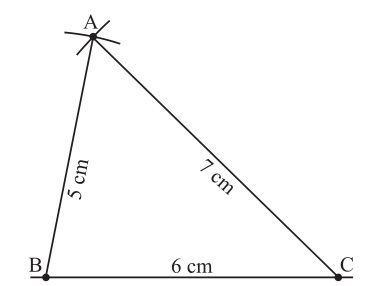
\includegraphics[width=5cm]{ncertProblemEnglish}
\end{center}

Consider the same problem from the Hindi version of the same book:\\

{\dn udAhrZ \rn{1}}\\
{\dn ek E/\7{B}j} ABC {\dn kF rcnA kFEje jbEk} AB = 5 {\dn s\?mF}, BC = 6 {\dn s\?mF} {\dn aOr} AC = 7 {\dn s\?mF} {\dn EdyA h\4}

{\dn hl}
\begin{enumerate}
\item 6 {\dn s\?mF} {\dn l\2bAI kA ek r\?KAK\2X} BC {\dn KF{\qva}Ece}\\
\item B {\dn ko k\?{\qva}\qb{d} mAnkr aOr} 5 {\dn s\?mF} {\dn E/>yA l\?kr ek cAp KF{\qva}Ece}\\
\item C {\dn ko k\?{\qva}\qb{d} mAnkr aOr} 7 {\dn s\?mF} {\dn E/>yA l\?kr ek cAp KF{\qva}Ece}\\
\item {\dn in cApo{\qva} k\? \3FEwEtQC\?d Eb\2\7{d} ko} A {\dn s\? a\2Ekt kFEje}\\
\item AB {\dn ko joEwe}\\
\item AC {\dn ko joEwe}\\
\end{enumerate}

\section{Related work}
\subsection{Anaphora}

Root, Rebecca Louise et al.~\cite{root-RL-86-phd-ut_semantics-of-anaphora-in-discourse} use the Discourse Representation Theory of Hans Kamp to develop a theory in which each sentence contributes to building a representation of the meaning of the discourse. They introduce ``reference markers'' for each noun phrase and truth is defined in terms of an embedding of the representation of the model. Along with the formal explanations, it is argued that this approach is attractive from a computational point of view.

Altaf Rahman and Vincent Ng~\cite{rahman-ng-11ijc_ensemble-based-coreference-resolution} use ensembles from a variety of supervised coreference models. They discuss different methods to apply a model-heterogenous ensemble for coreference resolution: ensemble-based methods significantly outperform the best member of the ensemble.

Nguyen et al.~\cite{nguyen-poesio-12coling_relational-coreference-resolution} use a filtering algorithm to rerank the output of coreference hypotheses, where the filter is based on relational structures between mentions and relationships. The second approach uses a joint model augmented with a set of relational features derived from semantic relationships of mentions. They claim improved performance of state-of-the-art coreference resolver based on learning.

Veselin Stoyanov et al.~\cite{stoyanov-eisneree-12coling_easy-first-coreference-resolution} build the coreference clusters incrementally, beginning with the most precise rules (termed as sieves by Raghunathan et al. (2010)) and use the available coreference information to guide the less precise sieves. Coreference resolution is inherently a global job. In this context, the approach of Raghunathan et al. (2010) may be taken as a rule-based greedy search for a globally consistent clustering.



\subsection{NLP and Parsing}
One of the most common techniques today to perform effective parsing is to use Part-of-Speech tagged language banks. Only few languages (about 8-10 of the 600+ languages in wide use) have the privilege of being resource-rich in the sense of having Penn-tree banks and other large-sized standardised corpus. An important observation is that fixed grammars, POS tags etc used in traditional parsers are not always the best way to break up a language. Taking a note of these shortcomings, we take a statistical approach to learn a language.

There has been a significant amount of work done on solving geometry construction problems. Gulwani et. al. \cite{gulwani2011synthesizing} propose a method that uses goal-based heuristic to simulate backward deduction to solve a problem expressed in a predefined logical construct. Schreck et. al. \cite{schreck2012geometric} talk about the same problem but use CAD methods to deal with constraints. At the same time, Itzhaky et. al. \cite{itzhaky2012solving} use the number of nondeterministic choices as a measure of a good solution. Ahmed, Umair et. al. \cite{ahmed2012can} look more into using domain-specific measures to minimize parser errors and augment the geometry problem solver, GeoSynth. All these papers have provided us with valuable insights into selecting important and expressive constructs for our intermediate language.

We summarize our observations in terms of following 3 parameters:
\begin{itemize}
\item Uses other linguistic/domain knowledge
\item Assumes linguistic cues are already translated into logical forms
\item Uses Parse knowledge
\end{itemize}

\begin{table}[H]
\smallskip
\begin{center}
\begin{tabular}{p{0.35\textwidth}p{0.20\textwidth}p{0.20\textwidth}p{0.20\textwidth}}
\hline
\bf{\small Paper} & \bf{\small Uses other linguistic/domain knowledge} & \bf{\small Assumes linguistic clues already traslated into logical forms} & \bf{\small Uses parse knowledge}\\[0.2cm]\hline
Schreck et. al.\cite{schreck2012geometric} & \texttt{YES} & \texttt{YES} & \texttt{NA}\\\\
Gulwani et. al.\cite{gulwani2011synthesizing} & \texttt{YES} & \texttt{YES} & \texttt{NA}\\\\
Itzhaky et. al.\cite{itzhaky2012solving} & \texttt{YES} & \texttt{YES} & \texttt{NA}\\\\
Ahmed et. al.\cite{ahmed2012can} & \texttt{YES} & \texttt{NO} & \texttt{YES}\\\\
Zettlemoyer et. al.\cite{zettlemoyer2012learning} & \texttt{YES} & \texttt{NO} & \texttt{YES}\\
\hline
\end{tabular}
\caption{Related Works}
\end{center}
\end{table}

Unlike all previous attempts, we do not assume that the logical forms of the sentences are available, nor we assume the availability of a parser. We use cross-lingual alignment to map the given sentence in natural language to metalanguage. It is therefore applicable to a large range of languages. We demonstrate this for two widely known languages belonging to very different families: Hindi and English.

\section{Design}
The interpreter consists of the following components:
\begin{itemize}
\item Aligner (training)
\item Grammar
\item Natural Language (NL) Interpreter
  \begin{itemize}
    \item NL to Metalanguage Mapper
    \item Heuristics-based Parser
    \item Semantics Analyser
    \item Plotter  
  \end{itemize}
\item Using Context to handle Anaphoras
\end{itemize}

\begin{figure}[H]
  \begin{center}
    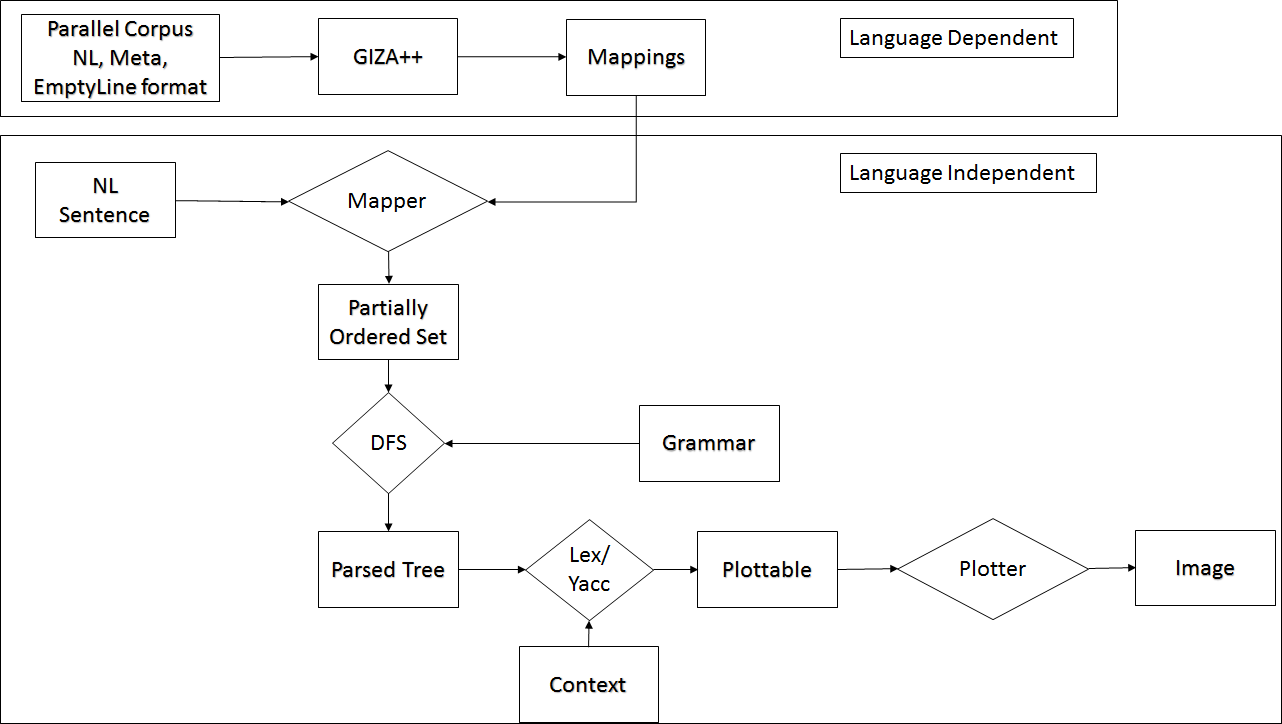
\includegraphics[scale=0.5]{workflow.png}
  \end{center}
  \caption{Work Flow}
  \label{}
\end{figure}


\subsection{Aligner}
Cross-lingual alignment is the heart of the learning mechanism in this project. It is used to obtain mapping/alignment between a natural language and our carefully designed and structured imperative metalanguage, L0. Since this alignment can be obtained for any natural language, the application is scalable to any number of natural languages.

We have used GIZA++ \cite{och2003systematic} as the cross-lingual aligner. GIZA++ is a statical machine translation toolkit that is used to train IBM Models 1-5 and an HMM word alignment model.

\subsubsection{Cross-Lingual alignment}
Cross-Lingual alignment is a technique to statistically align the words of a given pair of languages. It is close to translating one language into another, without any syntactic or semantic knowledge of any of the languages. As an example, for a pair of langauges, given sufficiently many sentences as illustrated in the table 2, a cross-lingual alignment assigns probabilities to the event that a particular source language token is mapped to a target language token.

\begin{table}[H]
\smallskip
\begin{center}
\begin{tabular}{p{0.33\textwidth}p{0.33\textwidth}p{0.33\textwidth}}
\hline
\vspace{0.1cm}\bf{English} & \vspace{0.1cm}\bf{Hindi} & \vspace{0.1cm}\bf{Meta Language}\\[0.2cm]\hline
Construct a line AB of length 4 cm & 4 {\dn s\?mF lMbAI kA ek r\?KAK\317wX} AB {\dn KF{\qva}Ece} & \texttt{construct lineSegment AB length 4 cm}\\[0.2cm]
With A as center and radius 3 cm, draw an arc & {\dn k\?{\qva}\qb{d}} A {\dn aOr E/>yA} 3 {\dn s\?mF l\?kr ek cAp KF{\qva}Ece} & \texttt{constrcut arc center A radius 3 cm}\\[0.2cm]
With B as center and radius 5 cm, draw an arc cutting the previously drawn arc at C & {\dn k\?{\qva}\qb{d}} B {\dn aOr E/>yA} 5 {\dn s\?mF l\?kr ek cAp KF{\qva}Ece jo phl\? KF{\qva}cF cAp ko} C {\dn kAVtA ho} & \texttt{construct intersectingArc center C radius 5 cm cuts arc previous at C}\\[0.2cm]
\hline
\end{tabular}
\caption{Sample Corpus}
\end{center}
\end{table}

\begin{table}[H]
\smallskip
\begin{center}
\begin{tabular}{p{0.33\textwidth}p{0.33\textwidth}c}
\hline
\bf{English} & \bf{Meta Language} & \bf{Probability}\\[0.2cm]\hline
Construct & \texttt{construct} & 1.00\\
Line segment & \texttt{lineSegment} & 1.00\\
intersects & \texttt{intersect} & 0.93\\
intersect eachother & \texttt{intersect} & 0.78\\
cut eachother & \texttt{intersect} & 0.87\\
cut & \texttt{cut} & 0.98\\
join & \texttt{join} & 1.00\\
mark & \texttt{mark} & 0.98\\
label & \texttt{mark} & 0.98\\
bisector & \texttt{bisector} & 0.60\\
interior & \texttt{interior} & 0.20\\
exterior & \texttt{exterior} & 0.20\\
\hline
\end{tabular}
\caption{Sample alignment between English and Metalanguage}
\end{center}
\end{table}

\begin{table}[H]
\smallskip
\begin{center}
\begin{tabular}{p{0.25\textwidth}p{0.25\textwidth}c}
\hline
\bf{Hindi} & \bf{Meta Language} & \bf{Probability}\\[0.2cm]\hline
{\dn lgA dFEjy\?} & \texttt{construct} & 0.90\\
{\dn KF{\qva}Ece} & \texttt{construct} & 0.98\\
{\dn rcnA kFEjy\?} & \texttt{construct} & 0.96\\
{\dn bnAiy\?} & \texttt{construct} & 0.98\\
{\dn r\?KAK\317wX} & \texttt{lineSegment} & 1.00\\
{\dn pr-pr \3FEwEtQC\?d} & \texttt{intersect} & 0.98\\
{\dn kAVtA ho} & \texttt{cut} & 0.82\\
{\dn kAV\?} & \texttt{cut} & 0.95\\
{\dn EmlAiy\?} & \texttt{join} & 0.98\\
{\dn joEwy\?} & \texttt{join} & 0.98\\
{\dn a\2Ekt kFEjy\?} & \texttt{mark} & 0.98\\
{\dn mAn lFEjy\?} & \texttt{mark} & 0.98\\
{\dn smE\392wBAjk} & \texttt{bisector} & 0.59\\
{\dn a<y\306wtr} & \texttt{interior} & 0.20\\
{\dn bEhBA\0g} & \texttt{exterior} & 0.20\\
\hline
\end{tabular}
\caption{Sample alignment between Hindi and Metalanguage}
\end{center}
\end{table}

\begin{figure}[H]
  \begin{center}
    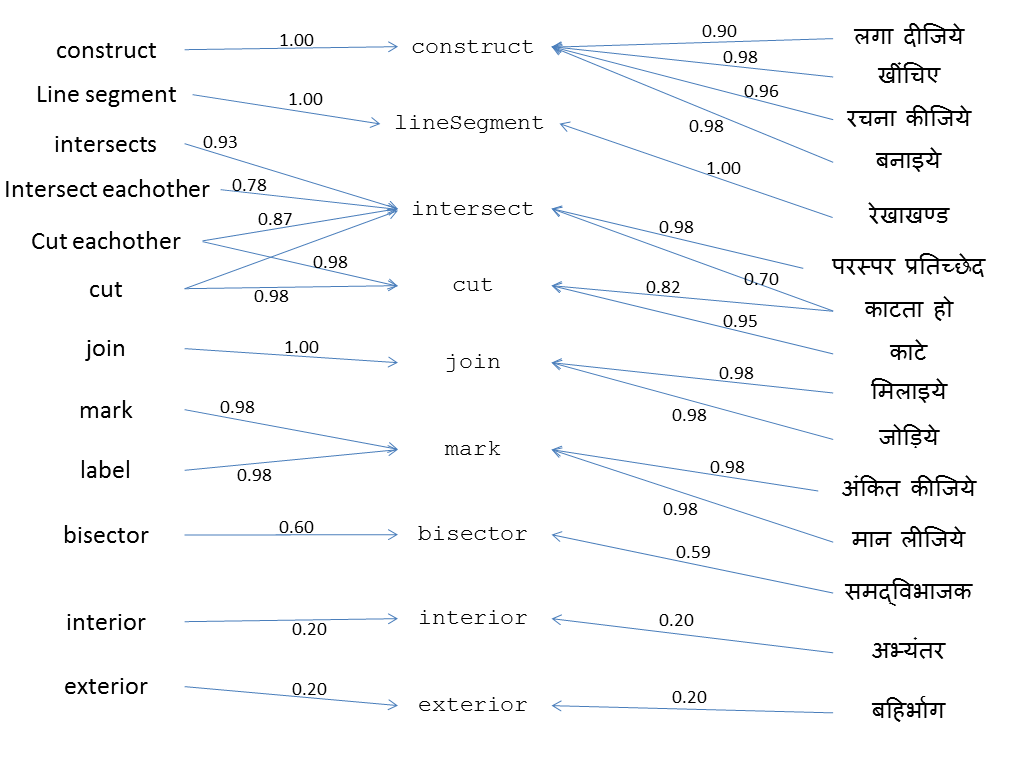
\includegraphics[scale=0.5]{image.png}
  \end{center}
  \caption{Graphical visualization of the sample alignment}
  \label{fig:pspic}
\end{figure}

\subsection{Grammar}
The grammar has been carefully designed to capture the underlying structure of the conventional (imperative) geometry construction steps. Note that there is a mild constraint on the grammar, which is a direct consequence of the assumption that the parameters of the object to be plotted occur near to parameter name in the input sentence. Hence the rules have been designed such that for each production rule, the leftmost non-terminal guides the search for the remaining non-terminals. [see section on Proximity]

\subsection{Natural Language (NL) Interpreter}

\subsubsection{NL to Metalanguage Mapper}
The interpreter component exploits the alignment model obtained from the Aligner component. Given a sentence expressed in a natural language, we use the alignment model to get the statistically most probable mapping of the NL sentence to a list of words in the language defined by the grammar. This list of words need not conform to a sentence in the language defined by the grammar but still carries some intent of the NL sentence, and hence can be called a partially ordered list of metalanguage words.

For example, in our problem, we obtain the following partially ordered set of words for the 6 steps in English:

\begin{enumerate}
\item \texttt{``construct line segment BC length 6 cm''}
\item \texttt{``B center construct arc radius 5 cm''}
\item \texttt{``C center construct arc radius 7 cm''}
\item \texttt{``mark intersection point these arcs A''}
\item \texttt{``join AB''}
\item \texttt{``join AC''}
\end{enumerate}

Similarly, following is the set for the 6 steps expressed in Hindi:
\begin{enumerate}
\item \texttt{``6 cm length line segment BC construct''}
\item \texttt{``B center 5 cm radius arc construct''}
\item \texttt{``C center 7 cm radius arc construct''}
\item \texttt{``these arcs intersection point A mark''}
\item \texttt{``AB join''}
\item \texttt{``AC join''}
\end{enumerate}

\subsubsection{Heuristics-based Parser}
At this stage, the parser takes the partially ordered set of words generated in the previous step and tries to map it to a sentence formed by the grammar. This is done by performing a DFS on the grammar tree and trying to fit every token in the set with some grammar terminal. Given any production rule, our DFS-based algorithm recursively expands the leftmost unexpanded nonterminal in the rule; on encountering a terminal, it tries to fit the terminal to some token near its parent's/left sibling's token. The subtrees which are not satisfied are pruned and search resumes with the next available production rule. The search is aided by the following heuristics:

\begin{enumerate}
\item \textbf{Proximity}\label{sec:proximity}\\
Proximity plays an important role in our parsing method e.g. we have assumed that the object that needs to be constructed would be near the ``construct'' word, and the length of a line segment would be near its name. Consider, as an example, ``\texttt{Construct a line segment AB of length 5 cm}''. Here, using our assumption we start searching for the object to be constructed near the ``construct'' word; it comes out to be the line segment AB. Note that we have to search on both the sides of the keyword (For corresponding hindi sentence, the set of words is ``\texttt{5 cm length line segment BC construct}''). This assumption is justified by the structure of the sentences in the natural languages, and specifically the geometry construction steps. This reduces the parsing complexity many-fold. As an another example, ``\texttt{Construct a line segment AB such that length of AB is equal to the difference of the length of CD and length of EF}''. Here, only those parse trees which demand the construction of AB are retained (as AB is nearer to ``construct'' than CD and EF); remaining trees which involve the construction of CD or EF are pruned.

\item \textbf{Type system}\\
The system is implicitly type-defined. For example, consider a statement like  ``\texttt{Mark a point A on it}''. Here ``it'' can be a line, line segment, circle etc. but not a point, as marking a point on a point is not permitted. Also, point pairs like AB would define a line segment or a ray, ABC would define an arc, 'l' would define a line (according to the conventions in the existing geometry texts). The grammar and the semantic analyser together form the type system.

\item \textbf{Validity of the output}\\
The search is also guided by the output produced at this stage. If the output produced seems correct, i.e., it uses most of the tokens in the set and conforms to some sentence generated by the grammar, it is passed to the semantic analyser. The semantic analyser then checks whether the output represents a valid intent to draw, i.e., a valid plottable object can be inferred out of it. If not, the parser tries to correct the parse tree starting from the rightmost leaf; this procedure is repeated until either we obtain something plottable or exhaust all the possibilities.

\end{enumerate}

For example, in our problem, the output sentences in the language defined by the grammar would be
\begin{enumerate}
\item ``\texttt{construct line segment BC length 6 cm}''
\item ``\texttt{construct arc center B radius 5 cm}''
\item ``\texttt{construct arc center C radius 7 cm}''
\item ``\texttt{mark intersection point these arcs A}''
\item ``\texttt{join AB}''
\item ``\texttt{join AC}''
\end{enumerate}

Note that, the output sentences for the hindi sentences would be the same, as the underlying grammar in which the parser tries to fit the sentences is the same.

\subsubsection{Semantics Analyser}
This stage of the parser uses Lex-Yacc to generate a set of primitive objects like points, lines, arcs etc. which need to be plotted in the last input construction step. All coordinates, radii, lengths and angles are resolved in this step. Anaphora are also resolved in this stage. This is detailed in the later sections.

The semantics analyser maintains two lists of plottables, one corresponding to the ``context'' (which is derived from the objects which were plotted in the previous construction steps) and ``diff'', which is generated from the current construction step and stores the objects which are to be plotted at this stage. At the end of the plotting step, the ``diff'' is appended to the ``context''. We put a restriction that is an object requires some primitive objects to be plotted, we require that such objects are either in the running context or in the ``diff'' list, e.g., a line segment construction would require the two points, which determine the line segment, to be plotted first. So these points with their coordinates are also stored in the ``diff'' list.

In the running example, after the first step, the generated diff list would be as follows:\\
\texttt{Points=\{B(0,0), C(6,0)\}, line segments=\{BC\}}

Similarly before the fifth step, the context would be:\\
\texttt{points=\{B(0,0), C(6,0), A(1,$\surd{24}$)\}, line segments=\{BC\}, arcs=\{(B,5), (C,7)\}}\\
and the diff would be\\
\texttt{line segments=\{AB\}}\\
The updated context after the fifth step would be\\
\texttt{points=\{B(0,0), C(6,0), A(1,$\surd{24}$)\}, line segments=\{BC, AB\}, arcs=\{(B,5), (C,7)\}}

The objects are arranged in the ``context'' and the ``diff'' list such that the last plotted object is at the end of the respective list. For a point which occurs for the first time in the construction step, and is independent of the running context, we assign a coordinate randomly.

\subsubsection{Plotter}
For each input construction step, the plotter receives a list of primitive objects from the semantic analyser and plots them on the canvas.

\subsection{Using Task Context to handle Anaphora}
An anaphora is a word or phrase which points back to a previously referred linguistic or semantic object.  Thus the anaphora and its antecedent both corefer to the same referent.

The semantics analyser uses the context (a list of objects which were plotted in the previous construction steps) to resolve the anaphoras. For example, consider the sentence ``\texttt{Mark a point M on it}''. Here ``it'' would refer to the most recently plotted markable object (objects on which a point can be marked e.g. lines, line segments, arcs, circles etc.). We fetch such markable object from the context to resolve the anaphora.

In case of the problem we consider, suppose we combine the fourth, fifth and the sixth step into ``\texttt{With B and C as centers and radii 5 and 7 cm, draw two arcs intersecting eachother at A}''. Here, ``arcs'' is the antecedent and ``eachother'' is the anaphora, both corefering to the same referent i.e. the arcs being drawn. Since the arcs have not been constructed yet, they are not in the task context. In this case, the semantic analyser comes to our rescue by providing for such sentences in the grammar.

At the same time, in the original fourth step, ``\texttt{mark intersection point these arcs A}'', the words ``these arcs'' guide us to fetch the last drawn arcs. The ''intersection point'' applied on ``these arcs'' yields us a markable object, which when combined with ``mark'' completes the parse.

By the fourth step, we obtain the following plot (Note that the dotted circles represent arcs):

\begin{figure}[H]
  \begin{center}
    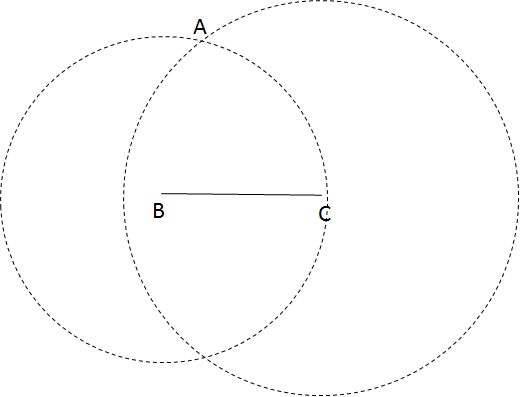
\includegraphics[scale=0.5]{step4.png}
  \end{center}
  \caption{Plot obtained after interpreting first four steps}
  \label{}
\end{figure}

If we join the fifth and the sixth step into ``\texttt{Join AB and AC}'', we get a case of ellipsis: the intent is to join AC too. Such cases are not handled here and are planned to be addressed in future.

By the sixth and the final step, we obtain the following plot:

\begin{figure}[H]
  \begin{center}
    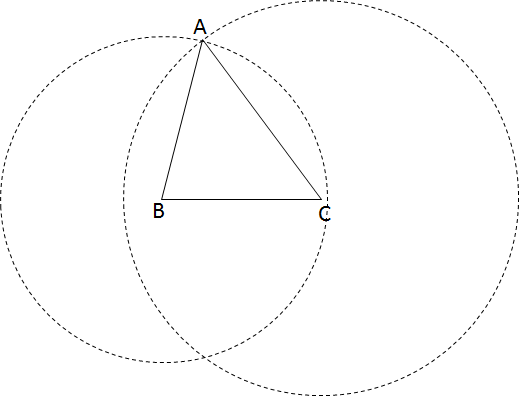
\includegraphics[scale=0.5]{step6.png}
  \end{center}
  \caption{Plot obtained after interpreting all the steps}
  \label{}
\end{figure}

\subsection{Language Independence}
Given a corpus in the specified format, the system generates a probabilistic mapping between the words in the language and the words in the meta language using cross-lingual alignment. This is then used in later stages to convert the presented sentence in the language to the meta language. After this conversion, the system behaves the same independent of the natutal language specified.

\section{Parsing metalanguage to generate plot}

The first input sentence in the English version of our problem is ``\texttt{Construct a line segment BC of length 6 cm}''. Using the English-to-Metalanguage map, we translate this sentence tokenwise to ``\texttt{construct line segment AB length 7 cm}'' where ``a'' and ``of'' map to empty words. Similarly, for the Hindi input sentence ``7 {\dn s\?mF lMbAI kA ek r\?KAK\317wX} AB {\dn KF{\qva}Ece}'', using the Hindi-to-Metalanguage map, we obtain the translation ``7 cm length line segment construct'', where ``{\dn kA}'' and ``{\dn ek}'' map to empty word.

Using heuristics-based parsing, we obtain the same parse tree for both of these translations:

\begin{figure}[H]
  \begin{center}
    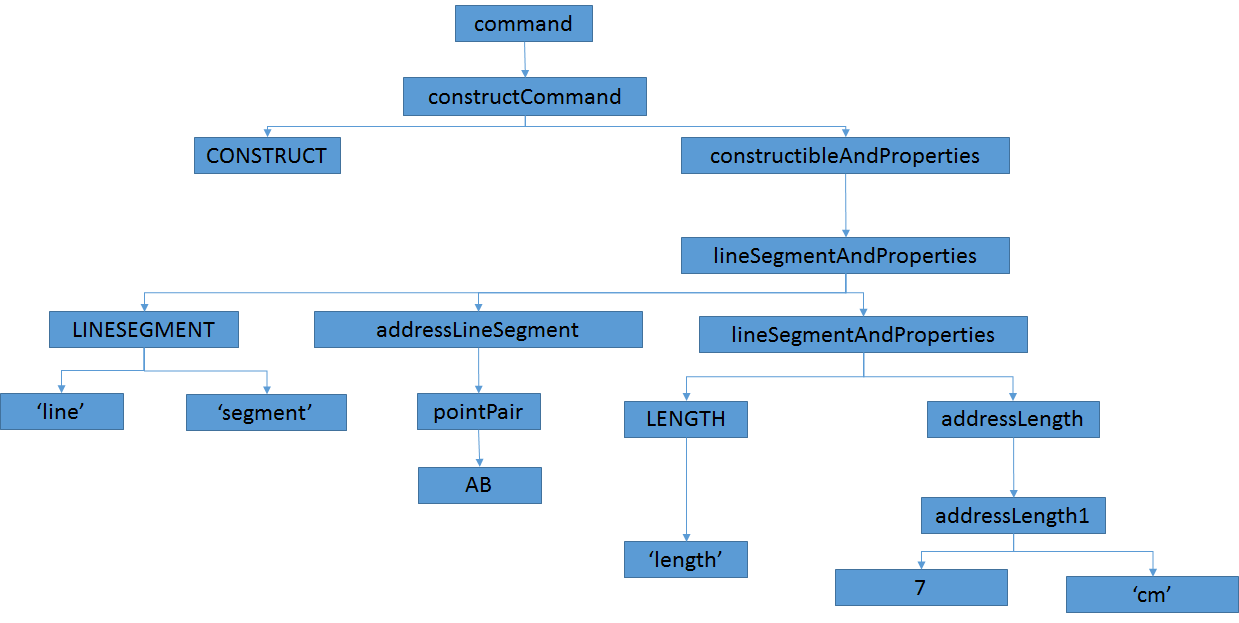
\includegraphics[scale=0.5]{parsetree.png}
  \end{center}
  \caption{Sample Parse Tree}
  \label{}
\end{figure}

The semantic analyser, which is, in reality, a lex-yacc parser, when presented with pre-order string of this parse tree, outputs a list of primitive objects to be plotted:

\texttt{points=\{B(0,0), C(6,0)\}, line segments=\{BC\}}

The plotter is a simple program which plots these geometric objects.

This approach has been shown to work for simple construction steps.

\section{Corpus Collection and Testing}

The corpus contains around 350 sentences from the geometry construction field in both the languages. These were collected from the NCERT textbooks of standards ${6^{th}}$ to ${9^{th}}$. English-Metalanguage and Hindi-Metalanguage sentence pairs were generated manually which were then used to train the cross lingual alignment software

The corpus has been formatted as follows:\\
For every sentence in natural language, 
\begin{itemize}
\item First line corresponds to the natural language sentence.
\item The second line corresponds to the intended meta langauge sentence.
\item The third line is an empty line.
\end{itemize}
The corpus is available at \cite{corpus}

To get an almost perfect probabilistic map between the parallel corpus, we impose a mild constraint: let the map be from language A to B; we design the corpus such that every word of the language A either maps to exactly one word of language B or to the empty word. Note that this is not necessary. It has been done so as to obtain the best possible map for a given corpus size under corss-lingual alignment. Poorer quality of map leads to considerable increase in the possible translations that the parser would have to parse.

\section{Results}
\begin{enumerate}
\item Number of sentences in the corpus: 360 each in English-to-Metalanguage and Hindi-to-Metalanguage corpus 
\item Number of unique tokens in each of the three languages are given below

\begin{table}[H]
\label{table:tokens}
\smallskip
\begin{center}
\begin{tabular}{cc}
\hline
\bf{Language} & \bf{Number of unique tokens}\\[0.2cm]\hline
English & 181+\\
Hindi & 169+\\
Metalanguage & 110+\\
\hline
\end{tabular}
\caption{Unique tokens in different languages}
\end{center}
\end{table}


\item The implementation demonstrates the performance of the system for atomic construction statements like ``\texttt{construct a line segment AB of length 5 cm}'' etc. Statements like ``\texttt{Construct an equilateral triangle of side length 5 cm}'', which involve more than one atomic step, have not been implemented.

The chapter on Geometry from CBSE NCERT Mathematics textbook for $6^{th}$ standard contains only the atomic construction steps, while chapters from $7^{th}$, $8^{th}$ and $9^{th}$ standard contain construction steps which require two or more applications of simple ruler-compass based (atomic) construction step.

Tabulated below is the performance of curent implementation. We are confident that the accuracy is bound to increase once the grammar and implementation is full-fledged.

\begin{table}[H]
\label{table:accuracy}
\smallskip
\begin{center}
\begin{tabular}{cccc}
\hline
\bf{Standard/Grade} & \bf{Corpus Size} & \bf{Number of successful parses} & \bf{Percentage}\\[0.2cm]\hline
$6^{th}$ & 84 & 77 & 91.67 \%\\
$6^{th}$ to $9^{th}$ & 225 & 172 & 76.44 \%\\
\hline
\end{tabular}
\caption{Unique tokens in different languages}
\end{center}
\end{table}

\end{enumerate}

\subsection{Failure Cases}

\begin{enumerate}

\item It is evident that sentences which are forbidden by the grammar can not be handled by the interpreter. This shortcoming can be easily removed by making the grammar more expressive, keeping in mind that it doesn't become ambiguous.

\item In cases such as ``\texttt{With A and B as centers, and radius as 4 and 5 cm, draw two arcs intersecting eachother at C}'', we see the ``B'' is nearer to the paramter ``centers'', while ``4'' is nearer to the parameter ``radius''. This guides the heuristics-based parser to draw two arcs with centers B and A and radius as 4 and 5 cm respectively; but the intent is to draw two arcs with centers A and B and radius as 4 and 5 cm respectively.

Clearly, if the sentence were ``\texttt{With centers as A and B, and radius as 4 and 5 cm, draw two arcs intersecting eachother at C}'', we would have captured the correct intent.

\end{enumerate}

\subsection{Difficulties \& Resolutions}
\begin{itemize}

\item {\bf Anaphoras}
Dealing with anaphoras like ``this'', ``it'', ``previous'', ``last'' etc in sentences like ``\texttt{Mark any point M on it}'', ``{\dn ek \7{s}EvDAjnk E/>yA l\?kr EpCl\? crZ vAl\? cAp ko Eb\306w\7{d}} A {\dn pr kAV\?{\qva}.}'' etc.\\ 
Anaphora are resolved by using the context (set of objects drawn in the previous steps).
\item {\bf Underspecified Parameters}
We also need to provide for unspecified radii, lengths and anlge measures e.g. ``\texttt{With A and B as centers and a suitable radius, draw two arcs interseting eachother at point C}''. \\
Radii, lengths etc. are supplied randomly in such cases, obeying the constraints which might have been put on such values in this or the previous step (e.g. ``\texttt{Construct a line segment with length greater than length of AB}'')

\item {\bf Probabilistic Mapping}
Since the mapping is statistical in nature, there might be various close alignments for the same source-language word. This forces us to resort to try out different possible alignments and look for the one that fits e.g. for the sentence ``\texttt{Construct AB of length 7.8cm}'', we get the following alignments with their corresponding probabilites (we assume that word-wise alignments are independent of eachother)\\
\begin{table}[H]
\begin{center}
\begin{tabular}{lc}
\hline
\bf{Mapped meta-language sentence} & \bf{Probability}\\\hline
\texttt{construct AB any length 7.8cm} & 0.716853\\
\texttt{construct AB lineSegment length} 7.8cm & 0.21081\\
\texttt{construct AB angle length 7.8cm} & 0.0723206\\
\texttt{construct AB center length 7.8cm} & 1.90645e-06\\
\hline
\end{tabular}
\caption{Map to possible metalanguage sentences alongwith their probabilities}
\end{center}
\end{table}
After incorporating the assumption that the every word in the sentence should map to either a word in the meta language or some null word, the map comes out to be nearly perfect. Even less frequent words like ``equilateral'', ``trapezium'' etc. map with very high probabilities with their meta langauge counterparts. This gives increased confidence in the correctness of meta langauge sentence produced from a given natural language sentence.
\end{itemize}

\subsection{Future Work}
\begin{enumerate}
\item Enrich the corpus as well as grammar to cover larger domains of expressions e.g. having larger number of primitive steps, providing for higher-level primitives, specifying relative distances, dealing with anaphoras and references
\item Expand the functionality of the system to work for all kinds of construction steps claimed so far
\item Deploy the system on a webserver to demonstrate its functionality and work towards making it more robust
\item In order to capture colloquial (non-academic) ways of expressing construction steps, we need to develop a user interface that augments the corpus with input sentences
\end{enumerate}

\nocite{schreck2012geometric}
\nocite{gulwani2011synthesizing}
\nocite{ahmed2012can}
\nocite{itzhaky2012solving}
\nocite{zettlemoyer2012learning}
\nocite{och2003systematic}
\nocite{root-RL-86-phd-ut_semantics-of-anaphora-in-discourse}
\nocite{kamp2011discourse}
\nocite{jurafsky2000speech}
\nocite{mitkov2002anaphora}

\renewcommand\refname{Annotated References}
\bibliography{report}{}
\bibliographystyle{plain-annote}
\end{document}
